\begin{figure}[t]
\centering
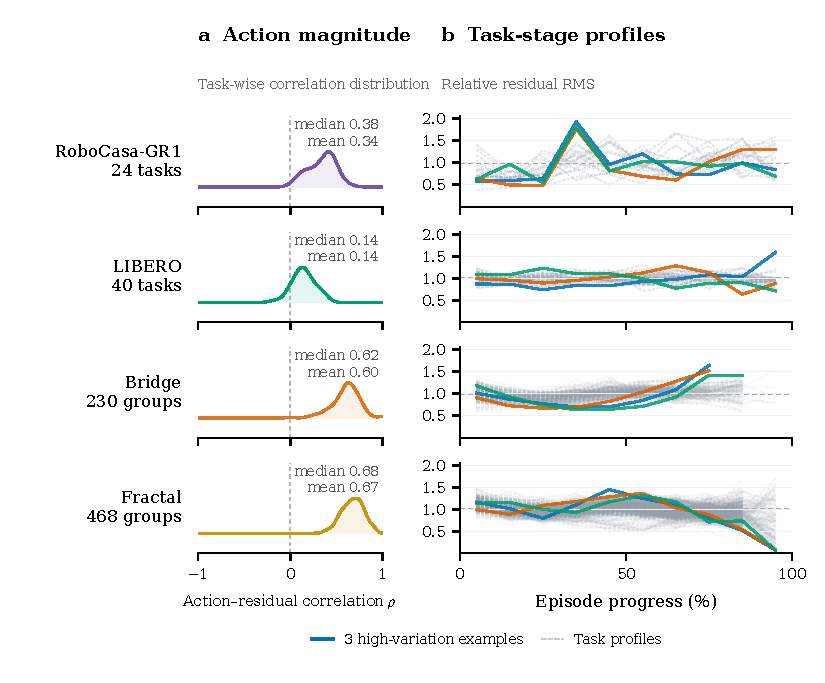
\includegraphics[width=\linewidth]{analysis/diagnostics/crossdataset_residual/all_datasets_progress_top3.pdf}
\caption{\textbf{Action magnitude and stage-dependent regression residuals across datasets.}
(a) Distributions of task-wise Spearman correlations between action RMS and general-MSE residual RMS. Curves are boundary-reflected kernel density estimates; annotations report the empirical median and mean over all qualifying tasks, weighted equally.
(b) Residual RMS across ten episode-progress bins, divided by each task's root-mean-square bin scale. Three tasks per dataset with the largest maximum-minus-minimum normalized stage-RMS range are highlighted as illustrative high-variation examples, not a random sample. Faint dashed lines show background task profiles; solid colored lines show the three selected task profiles, without temporal smoothing.
Points are plotted at bin centers (5\%--95\%); bins without valid full-action-chunk samples are omitted, so some curves end earlier.
Bridge and Fractal include nonempty instruction groups with at least 12 sampled demonstrations. These diagnostics use training-demonstration residuals.}
\label{fig:crossdataset-residual-clean}
\end{figure}
